\section{Sprint 8}

\subsection*{Summary}

\begin{table}[H]
	\centering
	\begin{tabular}{ll}
		\toprule
		\multicolumn{2}{c}{\textbf{Sprint 7}}\\
		\midrule
		\textbf{Periode} & 26.06.2015 12:00 Uhr\textendash 12.06.2015 20:00 Uhr\\
		\textbf{Stunden Soll} & \SI{216}{\hour}\\
		\textbf{Stunden Plan} & \SI{224}{\hour} \\
		\textbf{Stunden Ist} & \SI{255}{\hour}\\
		\bottomrule
	\end{tabular}
\end{table}

\begin{figure}[H]
	\centering
	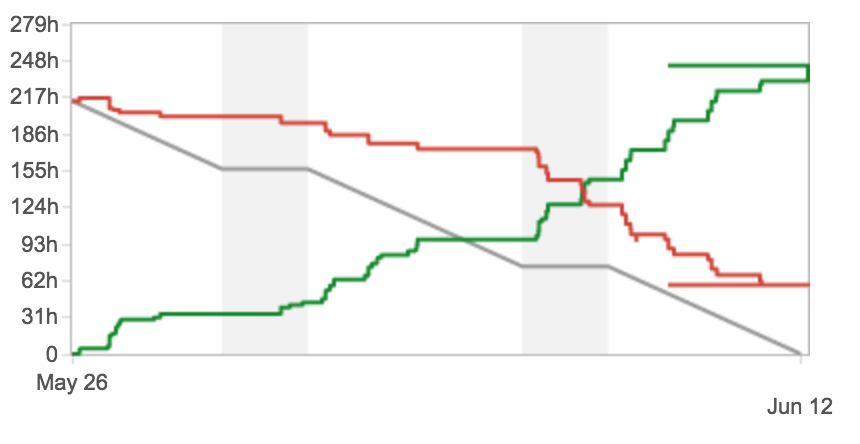
\includegraphics{fig/bd-sprint-8}
	\label{fig:pm:bd-sprint-8}
	\caption*{Burndown Chart Sprint 8}
\end{figure}

\subsection*{Ziele}
Dieser letzte, ausnahmsweise dreiwöchige Sprint dient der Finalisierung und Druck der Dokumentation sowie weitere mit der Bachelorarbeit zusammenhängenden organisatorischen Aufwände. Kleinere Last-Minute Bugfixes sind ebenfalls erlaubt.

\subsection*{Abgeschlossen}
Folgende High-level (ohne Subtasks) Jira Tasks wurden während Sprint 8 abgeschlossen. 

\begin{table}[H]	
\centering
\begin{tabular}{ll}
\toprule
\textbf{JIRA-Key} & \textbf{Summary}\\
\midrule
DAT-181 & Dokumentation\\
DAT-202 & Übrige Aufwände\\
DAT-203 & Projektmeeting\\
DAT-204 & Last Minute Bugfixes\\
DAT-207 & Organisation, Planung \& Kommunikation Sprint 8\\
\bottomrule
\end{tabular}	
\end{table}

\subsection*{Probleme}
Keine